\appendix
\section{One dimensional results}\label{sec:theory}

In this Appendix we show a convergence study in one space dimension
for both the first and second order accurate scheme.
We use the mesh from Figure 1(b) with two small cells
to the left and right of $U_0$. 
We solve the linear advection equation
\begin{equation}
u_t +  u_x = 0
\end{equation}
with periodic boundary conditions. 
The initial conditions are  one period of a cosine
wave. The domain goes from $[-1-\alpha {\textrm dx}, 1+\alpha \textrm{dx}]$.

The first order base scheme uses upwind differencing with Forward Euler,
and first order SRD. The second order scheme uses Heun's
method and second order accurate 
gradient reconstruction without limiters. 
In both cases, the state redistribution neighborhoods are the same, as shown in
Figure 1(b).
In this convergence study, we keep the volume fraction  of the small cell 
fixed at $\alpha=0.1$. This means the size of the domain changes as the mesh is
refined, and the mesh widths are not nicely divisible by 2.  We have taken 
account of this by scaling the $L_1$ error by the domain size 
of $2+2 \, \alpha \, \textrm{dx}$ to get error per unit length.

\hspace*{-.6in}
\begin{minipage}[c][4.5in][t]{3in}
{\small
\vspace*{-.5in}
%\begin{table}[h]
\begin{tabular}{|l|l|l|}\hline
\multicolumn{3}{|c|}{First Order Method} \\ \hline
$dx$ & $L_{\infty}$ error & $L_1$ error \\
 .15384E+00 &  .18213E+0  &  .10487E+0 \\
 .80000E-01 &  .82303E-01 &  .48000E-01 \\
 .40816E-01 &  .44043E-01 &  .26568E-01  \\
 .20618E-01 &  .20831E-01 &  .12846E-01 \\
 .10362E-01 &  .10506E-01 &  .65764E-02 \\
 .51948E-02 &  .51628E-02 &  .32578E-02 \\
 .26007E-02 &  .25851E-02 &  .16383E-02 \\
\hline \hline
\end{tabular}
\vspace*{.2in}
\begin{tabular}{|l|l|l|}\hline
\multicolumn{3}{|c|}{Second Order Method} \\ \hline
$dx$ & $L_{\infty}$ error & $L_1$ error \\
 .15384E+00 &  .27891E+0  & .17478E+0 \\
 .80000E-01 &  .84071E-01 & .52679E-01 \\
 .40816E-01 &  .21967E-01 & .13981E-01 \\
 .20618E-01 &  .57431E-02 & .36335E-02 \\
 .10362E-01 &  .14469E-02 & .92045E-03 \\
 .51948E-02 &  .36486E-03 & .23223E-03 \\
 .26007E-02 &  .91449E-04 & .58231E-04 \\
\hline \hline
\end{tabular}
}
%\end{table}
$\quad$ Table 3: {\sf  State redistribution errors for \\
graph at right.  }
\end{minipage}
\hspace*{.1in}
\vspace*{.1in}
\begin{minipage}[t][4.in][t]{3.in}
%\begin{figure}[h]
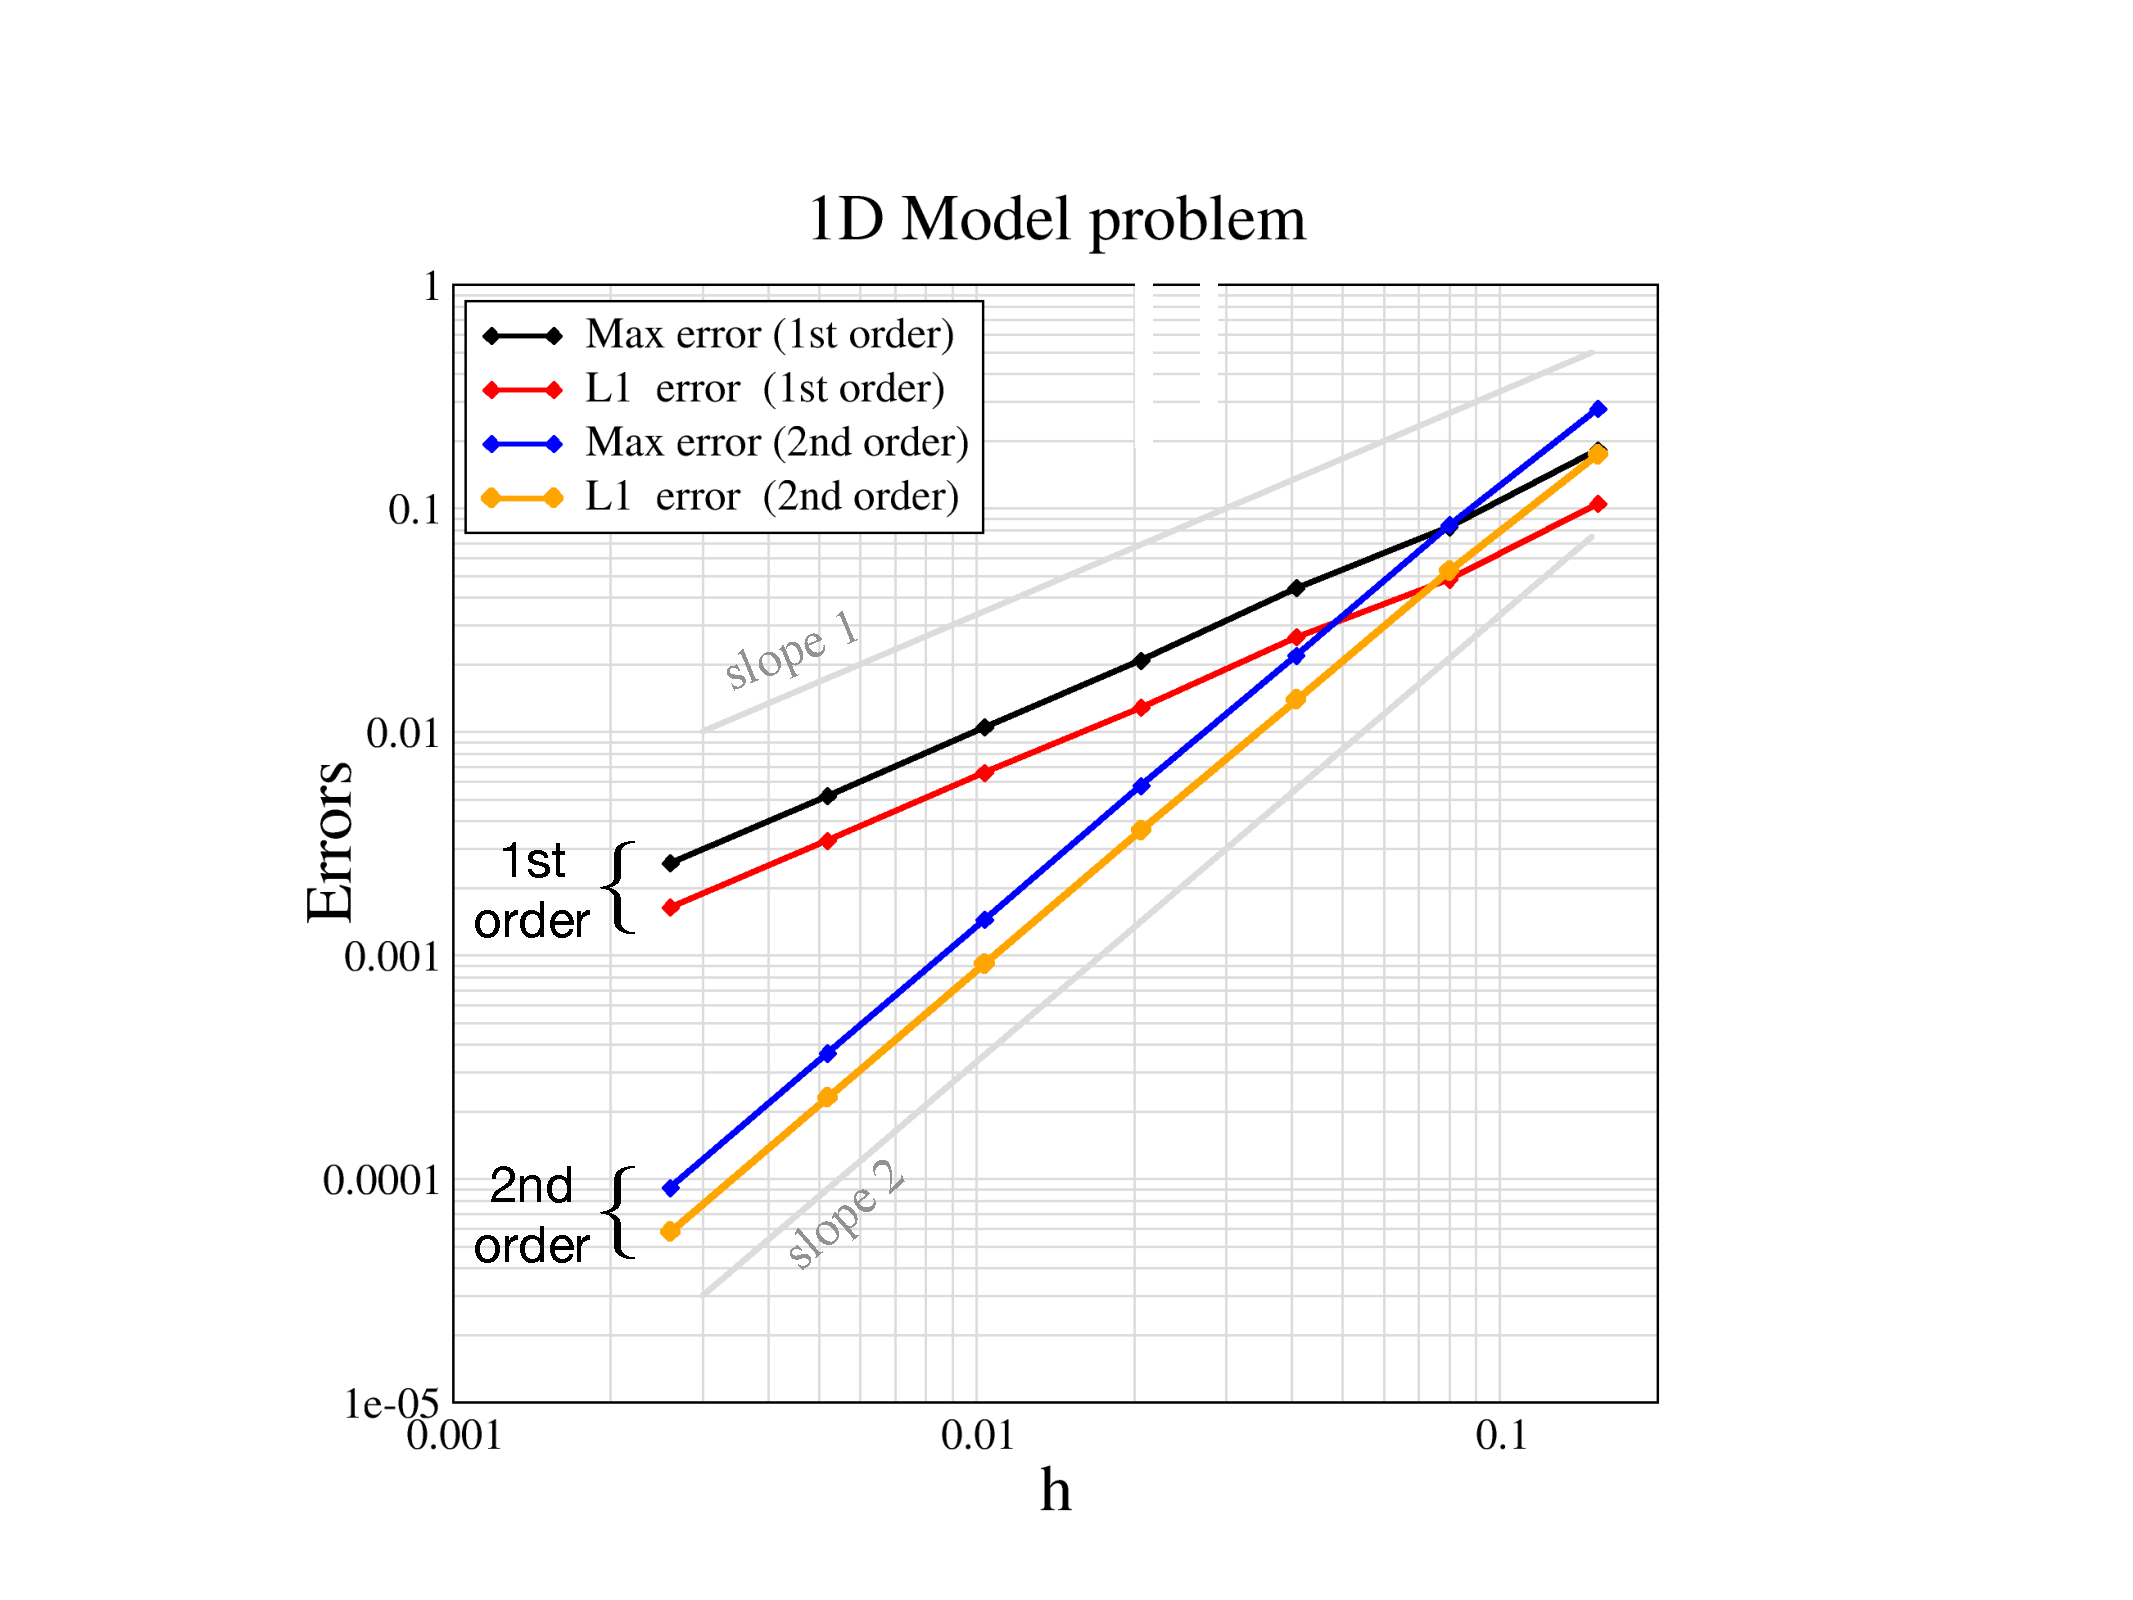
\includegraphics[height=3.0in]{figs/1dconvModel.pdf}
%\strut\vspace*{-\baselineskip}\newline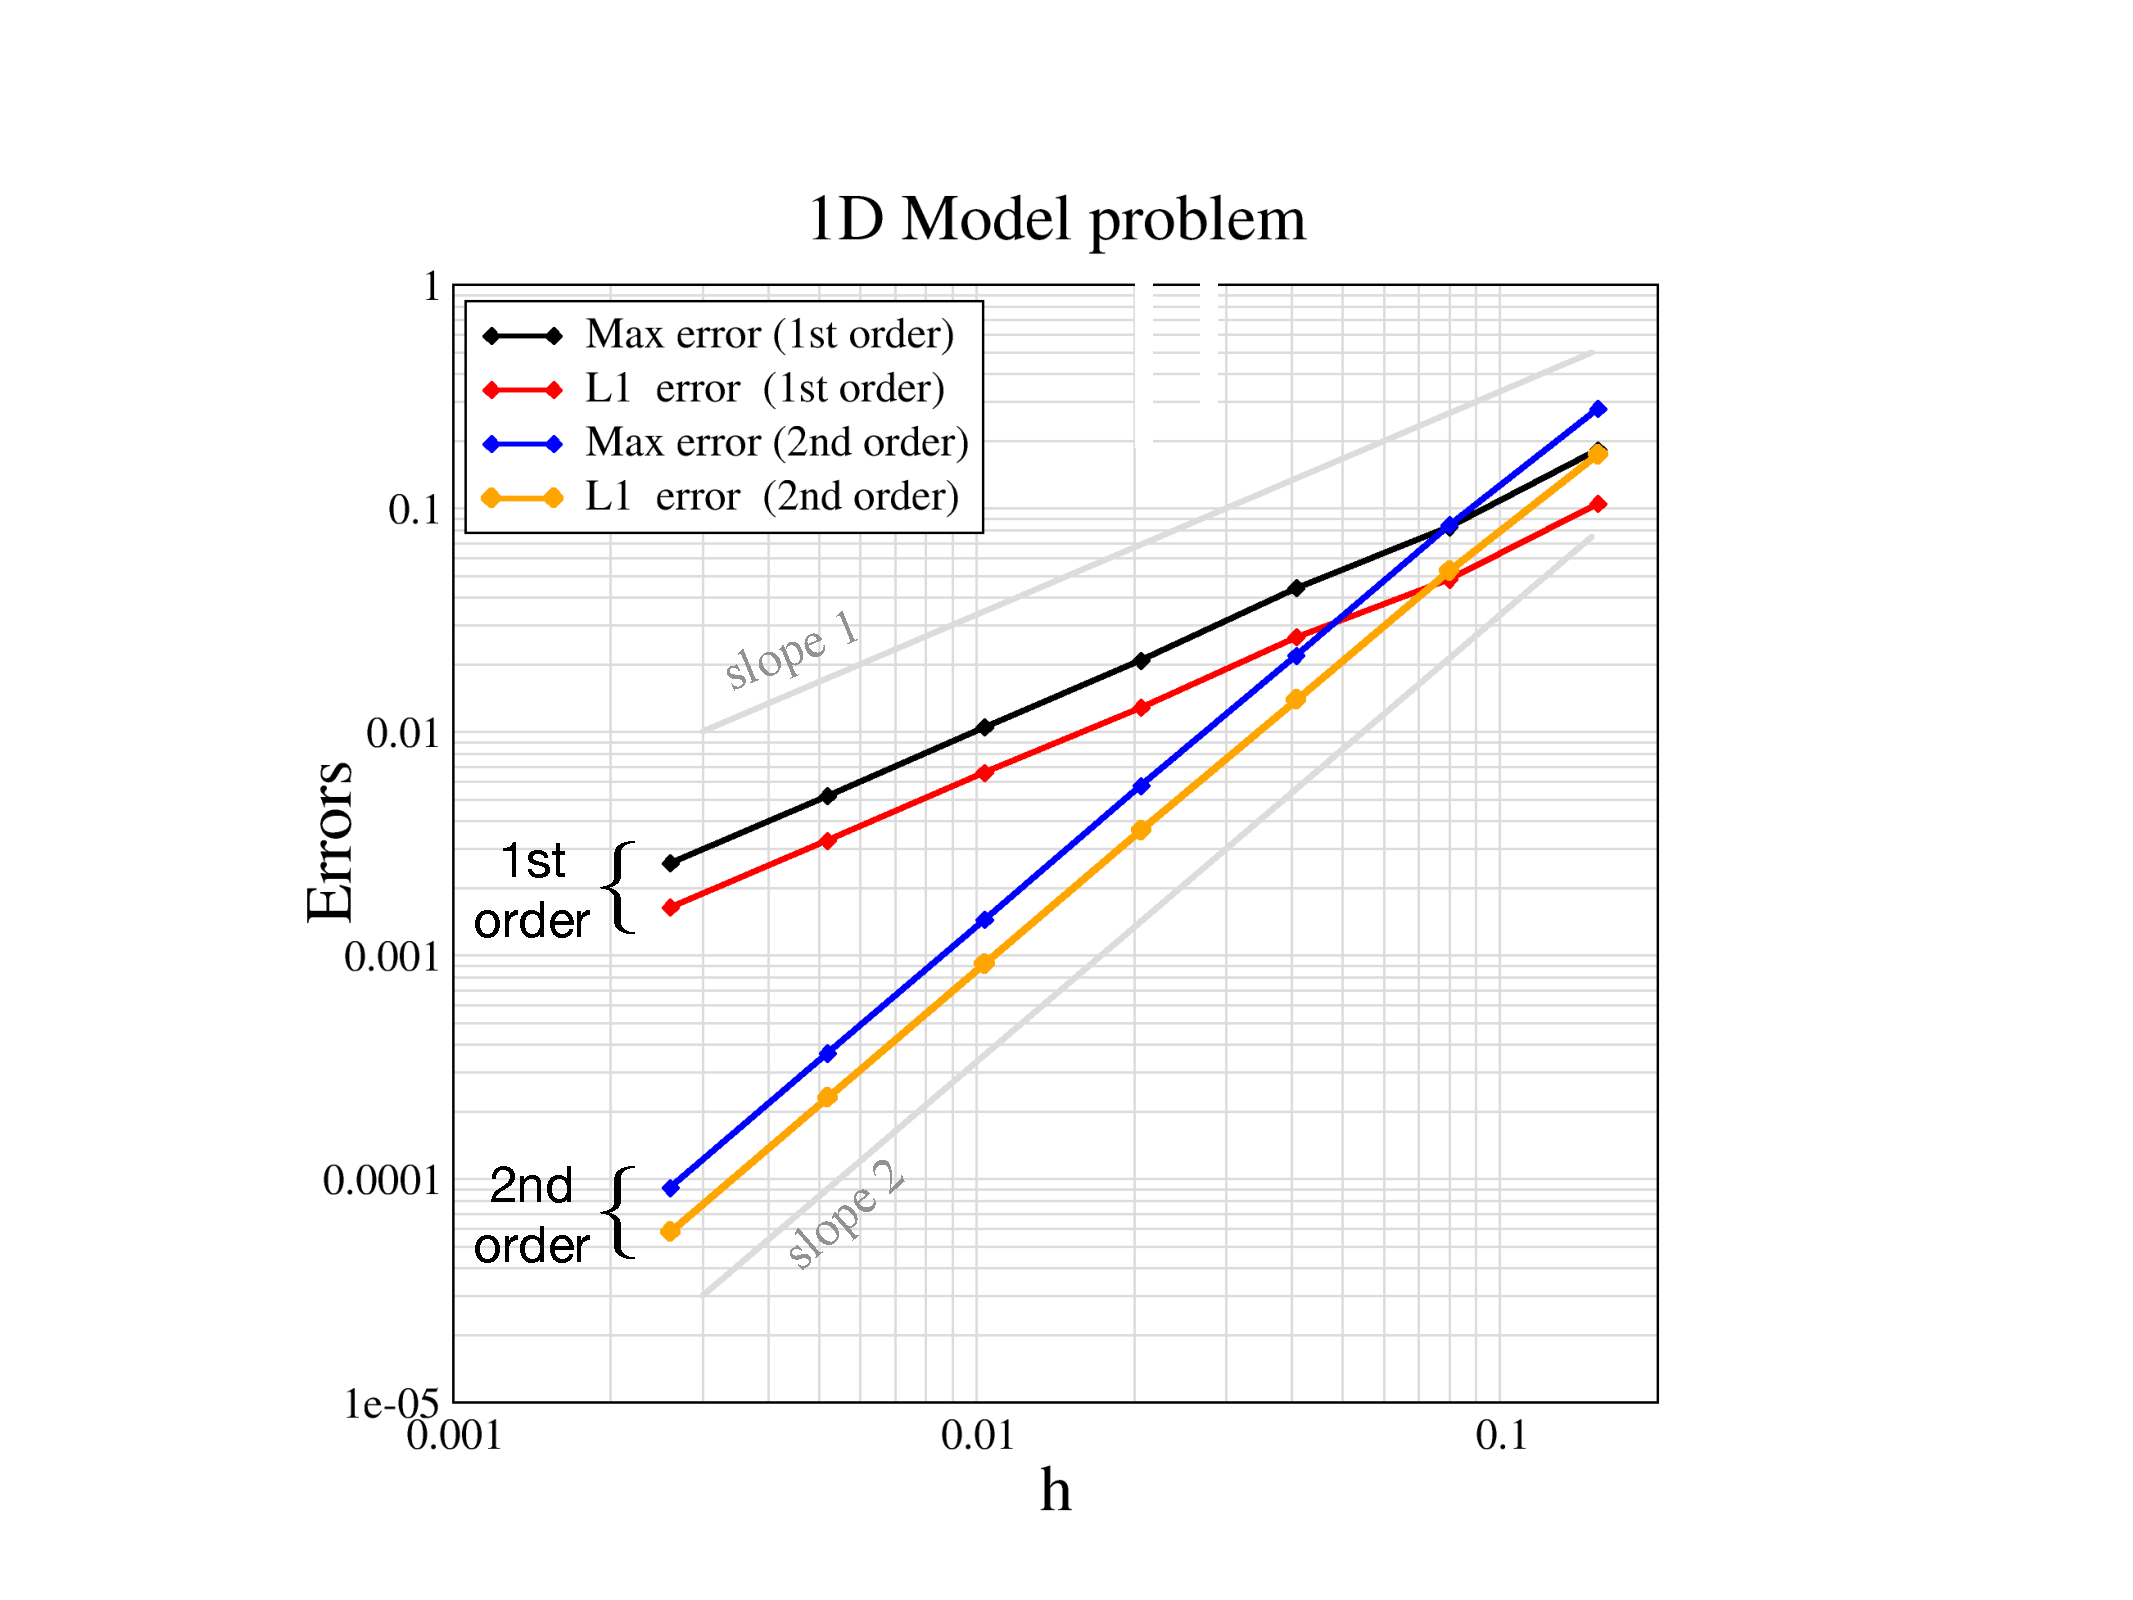
\includegraphics[width=\linewidth]{figs/1dconvModel.pdf}
%\caption{\sf  Convergence in the $l_{\infty}$ and  $L_1$ norms 
$\quad$ Figure 14: {\sf  Convergence in the $L_{\infty}$ and  $L_1$ norms 
for linear advection in one space dimension. 
SRD shows first and second order results as expected.  Exact numbers are in the table.
\label{fig:1dconv}}
%\end{figure}
\end{minipage}

We point out that these results are unique to one space dimension.
In two space dimensions we use normal merging neighborhoods, not
centered ones. Also the boundary is characteristic in the Euler
equations, and the error acumulates in a way that
does not occur in one dimension. Nevertheless it helps our
understanding to look at the convergence of these one dimensional examples. 
